\documentclass{article}
\usepackage[utf8]{inputenc}
\usepackage{tikz}
\usepackage{circuitikz}
\usepackage{geometry}
\usepackage{amsmath}
\usepackage{listings}
\usepackage{xcolor}
\geometry{margin=1in}
\title{Ultrasonic Sensor Documentation - Raspberry Pi 5 Integration}
\author{El Mehdi Adnani Kadmiri}
\date{July 17, 2025}

\begin{document}
	
	\maketitle
	
	\section{Description}
	The Ultrasonic Sensor (e.g., HC-SR04) uses ultrasonic sound waves to measure the distance between the sensor and an object. It sends out a sound pulse at 40kHz and measures the time taken for the echo to return. This time is then used to calculate distance using the speed of sound.
	
\section{Applications}

Ultrasonic sensors, such as the HC-SR04, are widely used in real-world scenarios where accurate, non-contact distance measurement is required. Their ability to detect objects using sound waves makes them ideal for various fields, including:

\begin{itemize}
	\item \textbf{Obstacle Detection:} Used in robotics and automation systems to detect and avoid objects.
	\item \textbf{Parking Assistance:} Commonly integrated into car bumpers to help drivers detect nearby obstacles while parking.
	\item \textbf{Liquid Level Monitoring:} Helps monitor fluid levels in tanks without direct contact, preserving sensor lifespan and hygiene.
	\item \textbf{Smart Waste Management:} Measures fill levels in garbage bins and sends data to optimize collection routes.
	\item \textbf{Industrial Automation:} Detects presence or absence of components on assembly lines to trigger actions.
\end{itemize}

	
	\section{Working Principle}
	The sensor has two main pins:
	\begin{itemize}
		\item \textbf{Trigger (TRIG)}: Sends an ultrasonic burst (10µs pulse).
		\item \textbf{Echo (ECHO)}: Receives the reflected wave and outputs a pulse proportional to distance.
	\end{itemize}
	Using the time between sending and receiving, distance is calculated with:
	\[
	\text{Distance (cm)} = \frac{\text{Time (µs)} \times 0.0343}{2}
	\]
	
	\section{Wiring Diagram}
	\begin{center}
		\begin{tabular}{|c|c|c|}
			\hline
			\textbf{Ultrasonic Pin} & \textbf{Raspberry Pi Pin} & \textbf{Function} \\
			\hline
			VCC & 5V & Power \\
			GND & GND & Ground \\
			TRIG & GPIO23 & Output Trigger Signal \\
			ECHO & GPIO24 & Input Echo Signal \\
			\hline
		\end{tabular}
	\end{center}
	\begin{center}
		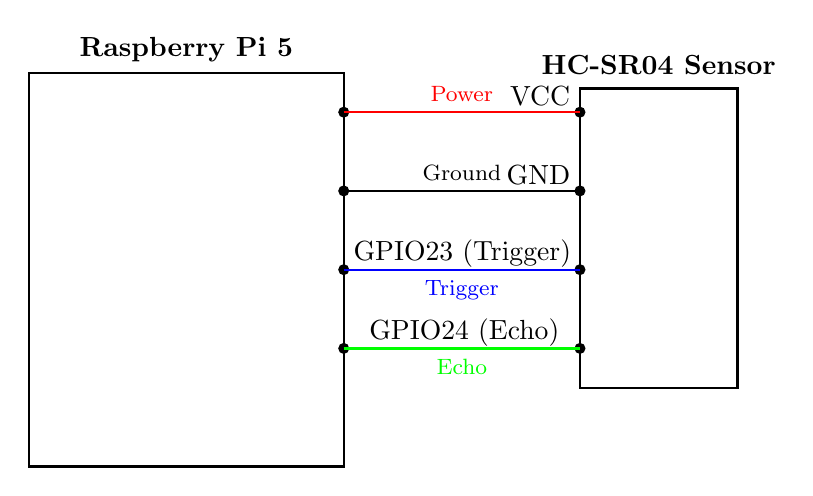
\begin{tikzpicture}
			
			% Raspberry Pi rectangle
			\draw[thick] (0,0) rectangle (4,5);
			\node at (2,5.3) {\textbf{Raspberry Pi 5}};
			
			% Sensor pin labels and dots
			\node[anchor=east] at (7,4.7) {VCC};
			\node[anchor=east] at (7,3.7) {GND};
			\node[anchor=west] at (4,2.7) {GPIO23 (Trigger)};
			\node[anchor=west] at (4.2,1.7) {GPIO24 (Echo)};
			\fill (4,4.5) circle (2pt); 
			\fill (4,3.5) circle (2pt);
			\fill (4,2.5) circle (2pt); 
			\fill (4,1.5) circle (2pt);
			
			% Ultrasonic sensor rectangle
			\draw[thick] (7,1) rectangle (9,4.8);
			\node at (8,5.1) {\textbf{HC-SR04 Sensor}};
			
			
			\fill (7,4.5) circle (2pt);
			\fill (7,3.5) circle (2pt);
			\fill (7,2.5) circle (2pt);
			\fill (7,1.5) circle (2pt);
			
			% Connecting wires
			\draw[red, thick] (4,4.5) -- (7,4.5) node[midway, above] {\footnotesize Power};
			\draw[black, thick] (4,3.5) -- (7,3.5) node[midway, above] {\footnotesize Ground};
			\draw[blue, thick] (4,2.5) -- (7,2.5) node[midway, below] {\footnotesize Trigger};
			\draw[green, thick] (4,1.5) -- (7,1.5) node[midway, below] {\footnotesize Echo};
			
		\end{tikzpicture}
	\end{center}
	
	\section{Libraries Used}
	\subsection*{Python: RPi.GPIO}
	\begin{itemize}
		\item Setup with: \texttt{import RPi.GPIO as GPIO}, \texttt{import time}
		\item Configure mode: \texttt{GPIO.setmode(GPIO.BCM)}
		\item Trigger pulse: \texttt{GPIO.output(TRIG, True)}
		\item Read echo: \texttt{GPIO.input(ECHO)}
	\end{itemize}
	
	\subsection*{C: wiringPi}
	\begin{itemize}
		\item Initialize GPIO: \texttt{wiringPiSetupGpio();}
		\item Set pins: \texttt{pinMode(TRIG, OUTPUT)}, \texttt{pinMode(ECHO, INPUT)}
		\item Control and read: \texttt{digitalWrite()}, \texttt{digitalRead()}, \texttt{micros()}
	\end{itemize}
	
	\section{Python Code Example}
	\begin{lstlisting}[language=Python]
		import RPi.GPIO as GPIO
		import time
		
		TRIG = 23
		ECHO = 24
		
		GPIO.setmode(GPIO.BCM)
		GPIO.setup(TRIG, GPIO.OUT)
		GPIO.setup(ECHO, GPIO.IN)
		
		GPIO.output(TRIG, False)
		time.sleep(2)
		
		GPIO.output(TRIG, True)
		time.sleep(0.00001)
		GPIO.output(TRIG, False)
		
		while GPIO.input(ECHO) == 0:
		pulse_start = time.time()
		
		while GPIO.input(ECHO) == 1:
		pulse_end = time.time()
		
		pulse_duration = pulse_end - pulse_start
		distance = (pulse_duration * 34300) / 2
		
		print("Distance: %.2f cm" % distance)
		GPIO.cleanup()
	\end{lstlisting}
	
	\section{C Code Example}
	\begin{lstlisting}[language=C]
		#include <wiringPi.h>
		#include <stdio.h>
		#include <stdlib.h>
		#include <sys/time.h>
		
		#define TRIG 23
		#define ECHO 24
		
		long getMicroseconds() {
			struct timeval tv;
			gettimeofday(&tv, NULL);
			return tv.tv_sec * 1000000 + tv.tv_usec;
		}
		
		int main(void) {
			if (wiringPiSetupGpio() == -1)
			return 1;
			
			pinMode(TRIG, OUTPUT);
			pinMode(ECHO, INPUT);
			
			digitalWrite(TRIG, LOW);
			delay(500);
			
			digitalWrite(TRIG, HIGH);
			delayMicroseconds(10);
			digitalWrite(TRIG, LOW);
			
			while (digitalRead(ECHO) == LOW);
			long start = getMicroseconds();
			
			while (digitalRead(ECHO) == HIGH);
			long end = getMicroseconds();
			
			long duration = end - start;
			float distance = duration * 0.0343 / 2;
			
			printf("Distance: %.2f cm\n", distance);
			return 0;
		}
	\end{lstlisting}
	
	\section{Conclusion}
	The Ultrasonic Sensor provides accurate, non-contact distance measurement and is widely used in robotics. With basic GPIO and timing functions, it integrates well with the Raspberry Pi using both Python and C.
	
\end{document}
